\section{Research abroad}\label{abroad}

During the PhD I was a as visiting researcher in two foreign institutions: \emph{City London University}\footnote{City London University - http://city.ac.uk} in London (UK) and \emph{MIT SENSEable City Lab}\footnote{MIT SENSEable City Laboratory - http://senseable.mit.edu} in Boston, MA (USA). The purpose of the two visits was to investigate whether the technologies developed during the PhD could be generalised to application domains that share similarities with crisis training.

During fourteen weeks spent as visiting fellow at City University I investigated the design and production of \emph{Hazel Court}, a digitally augmented serious game for training of dementia carers for better care. I worked under the supervision of professor Neil Maiden. A working prototype of \emph{Hazel Court} (Figure \ref{fig:hazel-court}) has been implemented and evaluated in eight care homes in the greater London area. The game design and underpinning theories are reported in a joined publication to be submitted. This experience strengthened my competences in building sensing based-interfaces to support reflection in a domain which shares similarities with crisis training. It added to the study of RQ2 and RQ3.
\begin{figure}
	[h] \centering 
	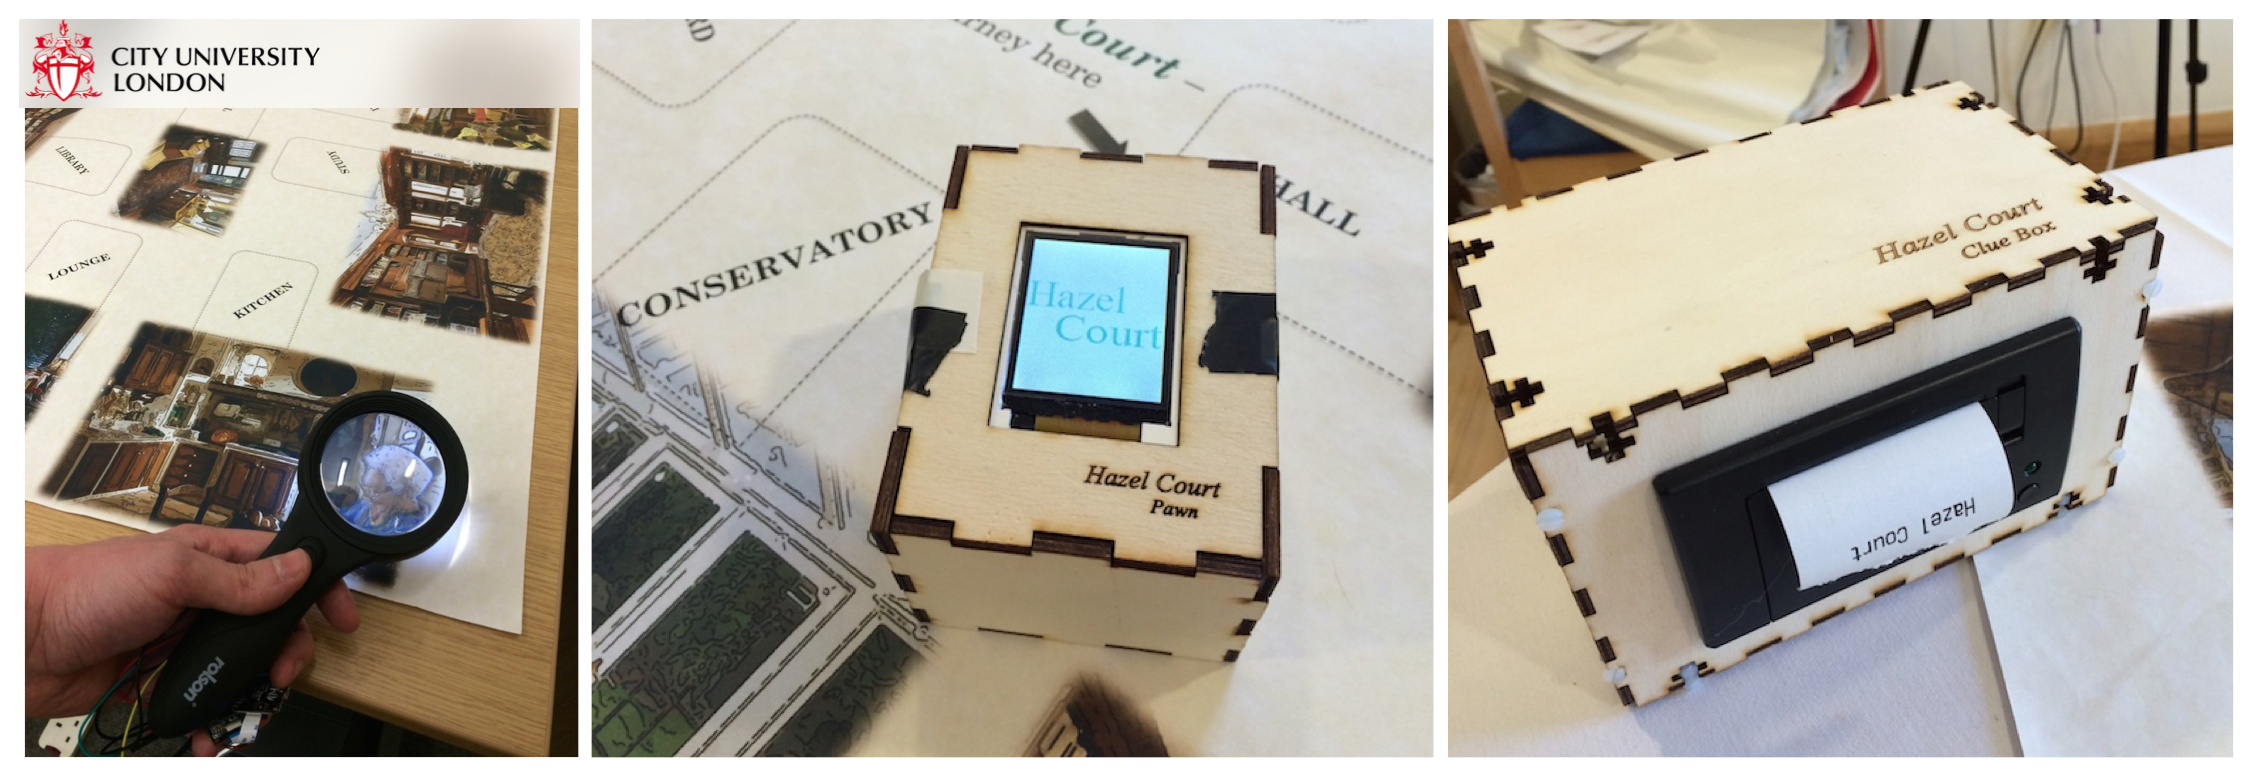
\includegraphics[width=1
	\textwidth]{city} \caption{The Hazel Court prototype} \label{fig:hazel-court} 
\end{figure}

During twelve weeks spent as visiting fellow at the MIT SENSEable City Lab I investigated the design and production of a tangible interface to promote user engagement and reflection about urban-mobility data. I worked under the supervision of professor Carlo Ratti. A working prototype of \emph{DriveWAVE} (Figure \ref{fig:drivewave}) has been implemented. DriveWAVE is a tangible interface that allows casual players in public spaces to challenge a computer brain against managing car flows towards minimizing pollution and avoiding traffic jams. The installation aims at sparking the interest in future sustainable cities\footnote{For more information please visit http://senseable.mit.edu/wave/}. The prototype features sensing-based interaction with the audience via presence sensors, physical controllers and digital projections. The work has been displayed to the public in two exhibitions: ``Wave'' held in Paris and ``CNR Internet Festival'' held in Pisa, Italy. This experiences streghtned my competences in building complex sensing-based systems to be deployed in public settings and added to the investigation of RQ3.
\begin{figure}
	[h] \centering 
	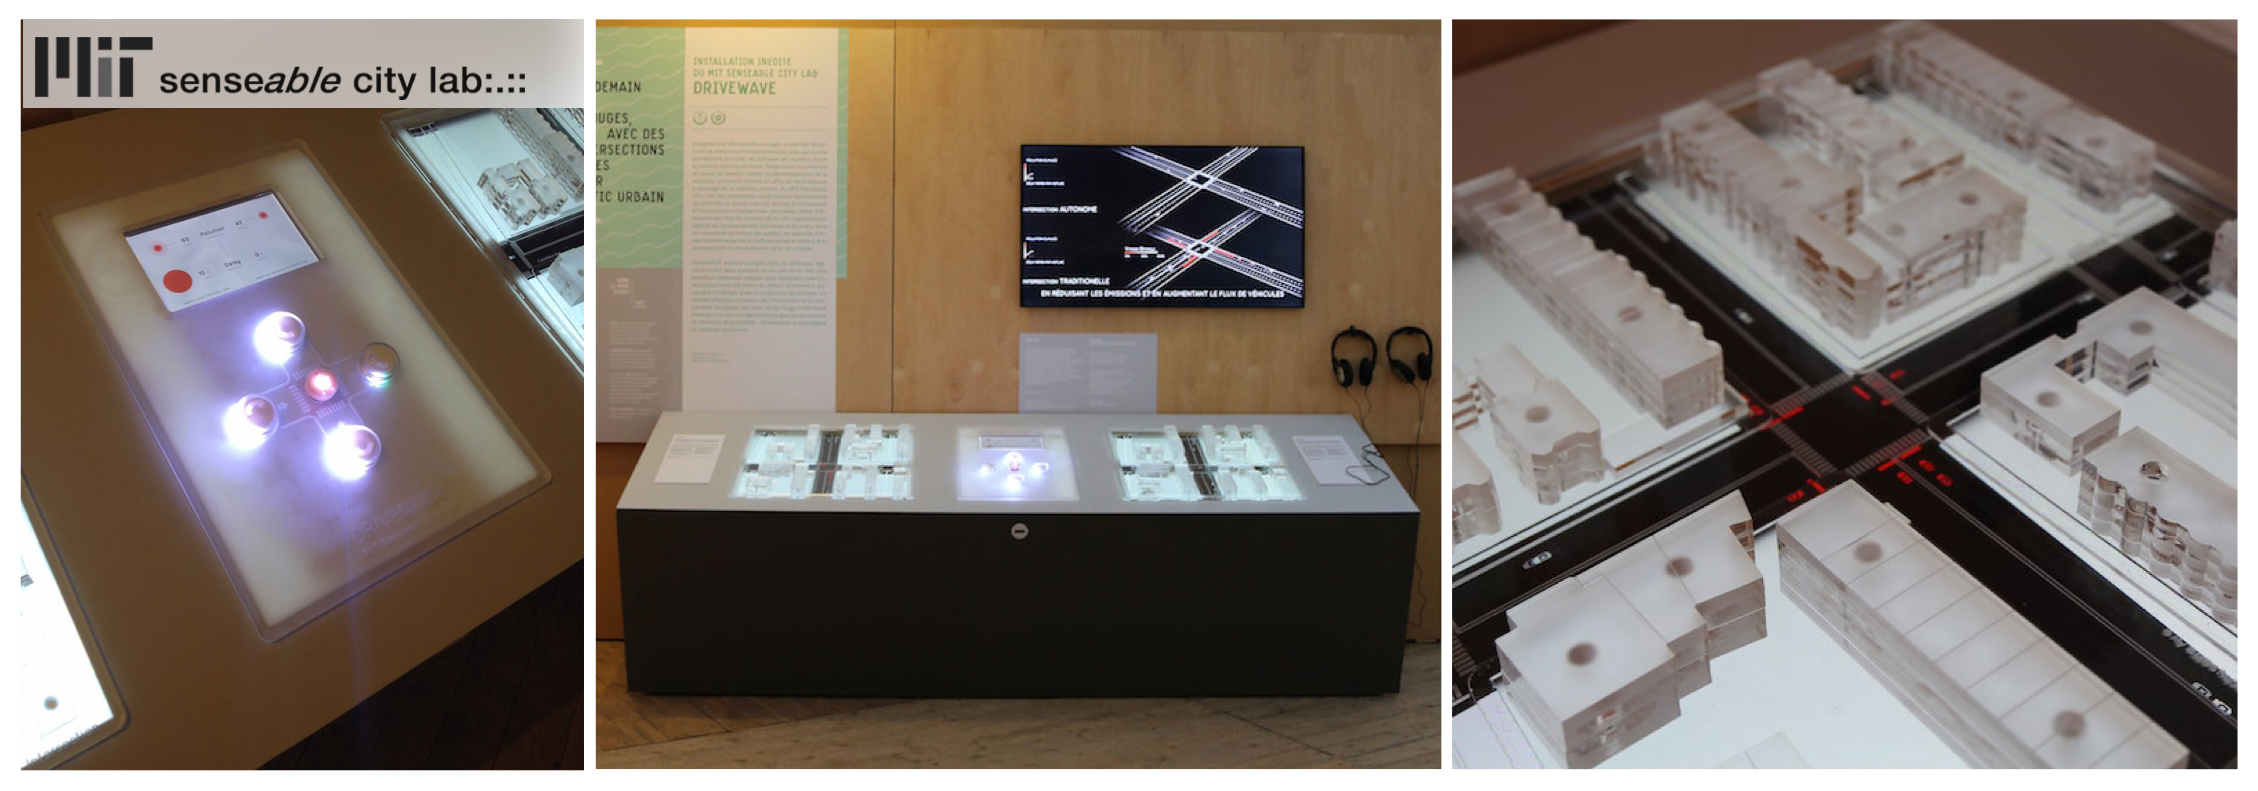
\includegraphics[width=1
	\textwidth]{mit} \caption{The DiveWAVE prototype} \label{fig:drivewave} 
\end{figure}